\noindent
It is a generally accepted convention that $0^0=1$.
By drawing a graph of the function $f(x)=|x^x|$ we can see why this
convention makes sense.
Of course, we want to draw the absolute value, or magnitude of $x^x$ because
$x^x$ is mostly complex when $x<0$.

\medskip
\verb$f=abs(x^x)$

\verb$xrange=(-2,2)$

\verb$yrange=(-2,2)$

\verb$draw(f)$

\begin{center}
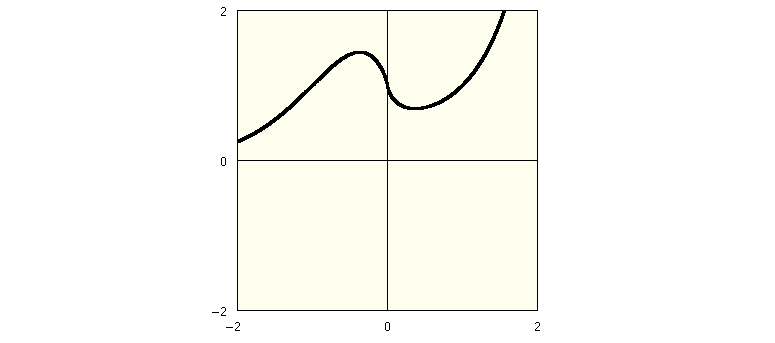
\includegraphics[scale=0.4]{zerozero.png}
\end{center}

\medskip
\noindent
We can see how $0^0=1$ results in a continuous line through $x=0$.

% What are the coordinates for the local minimum and maximum seen above?
